%%%%%%%%%%%%%%%%%%%%%%%%%%%%%%%%%%%%%%%%%%%%%%%%%%%%%%%%%%%%%%%%%%%%%%%%%%%%%%%%
% AMS Beamer series / Bologna FC / Template
% Andrea Omicini
% Alma Mater Studiorum - Università di Bologna
% mailto:andrea.omicini@unibo.it
%%%%%%%%%%%%%%%%%%%%%%%%%%%%%%%%%%%%%%%%%%%%%%%%%%%%%%%%%%%%%%%%%%%%%%%%%%%%%%%%
%\documentclass[handout]{beamer}\mode<handout>{\usetheme{default}}
%
\documentclass[presentation, 9pt]{beamer}\mode<presentation>{\usetheme{AMSBolognaFC}}
%\documentclass[handout]{beamer}\mode<handout>{\usetheme{AMSBolognaFC}}
%%%%%%%%%%%%%%%%%%%%%%%%%%%%%%%%%%%%%%%%%%%%%%%%%%%%%%%%%%%%%%%%%%%%%%%%%%%%%%%%
\usepackage[T1]{fontenc}
\usepackage{wasysym}
\usepackage{amsmath,blkarray}
\usepackage[minted,most]{tcolorbox}
\usepackage{centernot}
\usepackage{fontawesome}
\usepackage{fancyvrb}
\usepackage{minted}
\usepackage{hyperref}
\usepackage{multicol}
\setminted[scala]{fontsize=\scriptsize,baselinestretch=1,obeytabs=true, tabsize=2}
\usepackage[ddmmyyyy]{datetime}
\setminted{fontsize=\footnotesize}
\renewcommand{\dateseparator}{}
%\renewcommand{\thefootnote}{\fnsymbol{footnote}}
\newcommand{\version}{1}
\usepackage[
	backend=biber,
	citestyle=authoryear-icomp,
	maxcitenames=1,
	bibstyle=numeric]{biblatex}

	\makeatletter

\addbibresource{biblio.bib}
%%%%%%%%%%%%%%%%%%%%%%%%%%%%%%%%%%%%%%%%%%%%%%%%%%%%%%%%%%%%%%%%%%%%%%%%%%%%%%%%
\title[Reinforcement Learning]
{Reinforcement Learning}
\subtitle{Unlocking the Power of AI Agents}
%
%
\author[\sspeaker{Aguzzi}]
{\speaker{Gianluca Aguzzi} \href{mailto:gianluca.aguzzi@unibo.it}{gianluca.aguzzi@unibo.it}}
%
\institute[DISI, Univ.\ Bologna]
{Dipartimento di Informatica -- Scienza e Ingegneria (DISI)\\
\textsc{Alma Mater Studiorum} -- Universit{\`a} di Bologna \\[0.5cm]
\textbf{Talk @} \bold{Advanced School in Artificial Intelligence (ASAI)}}
%
\renewcommand{\dateseparator}{/}
\date[\today]{\today}
%
\AtBeginSection[]
{
  \begin{frame}
  \frametitle{Contents}
  \tableofcontents[currentsubsection, 
	sectionstyle=show/shaded, 
	subsectionstyle=show/shaded]
  \end{frame}
}
\AtBeginSubsection[]
{
  \begin{frame}
  \frametitle{Contents}
  \tableofcontents[currentsubsection, 
	sectionstyle=show/shaded, 
	subsectionstyle=show/shaded]
  \end{frame}
}
%%%%%%%%%%%%%%%%%%%%%%%%%%%%%%%%%%%%%%%%%%%%%%%%%%%%%%%%%%%%%%%%%%%%%%%%%%%%%%%%
\begin{document}
%%%%%%%%%%%%%%%%%%%%%%%%%%%%%%%%%%%%%%%%%%%%%%%%%%%%%%%%%%%%%%%%%%%%%%%%%%%%%%%%

%/////////
\frame{\titlepage}
%/////////
\begin{frame}{}
	\begin{columns}
		\begin{column}{0.5\textwidth}
		\centering
		\fbox{
\includegraphics[width=0.5\linewidth]{img/me.jpeg}}
		\\
		\vspace{0.2cm}
		\href{https://github.com/cric96}{\faGithub} \,
		\href{https://stackoverflow.com/users/10295847/gianluca-aguzzi}{\faStackOverflow} \,
		\href{https://www.linkedin.com/in/gianluca-aguzzi-265998170/}{\faLinkedin} \,
		\href{https://www.unibo.it/sitoweb/gianluca.aguzzi}{\faGlobe} \,
		\end{column}
		\begin{column}{0.5\textwidth}
			\begin{itemize}
				\item PhD student in Computer Science and Engineering
				\item Research interests:
				\begin{itemize}
					\item Multi-agent systems
					\item Distributed Collective Intellingence
					\item Deep Reinforcement Learning
					\item Multi-agent Reinforcement Learning
					%\item Distributed Macro-programming
				\end{itemize}
				%\item Lead developer of \href{https://scafi.github.io/}{ScaFi}
				%\item Scala Lover \& Functional Programming enthusiast
			\end{itemize}
		\end{column}
	\end{columns}
\end{frame}
\begin{frame}{Resources}
\begin{itemize}
	\item \emph{An Introduction to Reinforcement Learning}, Sutton and Barto,1998
	\begin{itemize}
		\item Available online at \url{http://incompleteideas.net/book/the-book-2nd.html}
	\end{itemize}
	\item \emph{Foundations of Deep Reinforcement Learning: Theory and Practice in Python}, Laura Graesser and Wah Loon Keng, 2020
	\item \emph{Deep Mind Lectures}:
	\begin{itemize}
		\item \textbf{Introduction to Reinforcement Learning with David Silver}: \url{https://www.deepmind.com/learning-resources/introduction-to-reinforcement-learning-with-david-silver}
		\item \textbf{Reinforcement Learning Lecture Series}: \url{https://www.deepmind.com/learning-resources/reinforcement-learning-lecture-series-2021}
	\end{itemize}
\end{itemize}
\end{frame}
%===============================================================================
\section{Introduction}
%===============================================================================
\begin{frame}[plain,c]
	%\frametitle{A first slide}
	\begin{center}
	\Huge What is Reinforcement Learning?
	\end{center}
\end{frame}

\begin{frame}[plain,c]
	%\frametitle{A first slide}
	\begin{center}
	\Huge What is Intelligence?
	\\
	\huge \emph{\textbf{learning} to make \textbf{decisions} to achive \textbf{goals}}
	\end{center}
\end{frame}
\begin{frame}{What is Reinforcement Learning?}
\begin{itemize}
	\item Animals learn by interacting with our environment
	\begin{itemize}
		\item Babies learn how to communicate by interacting with parents
		\item Dogs learn how to behave by following the owner's orders
		\item Me learn how to surfing by falling from the surfboard
	\end{itemize}
	\item Difference from supervised learning:
	\begin{itemize}
		\item \textbf{active} learning (learn by doing)
		\item \textbf{sequential} interaction 
		\item \textbf{delayed} feedback
	\end{itemize}
	\item Learning guided by \textbf{goal} (goal-directed)
	\item Learning without examples \faArrowRight \, guided by reward signal
\end{itemize}
\end{frame}

\begin{frame}{Interaction loop}
\centering
\Large An \textbf{agent} interacts with the \textbf{environment} by perceive an \textbf{observation} and take an \textbf{action} accordingly which leads to a \textbf{reward}
\\
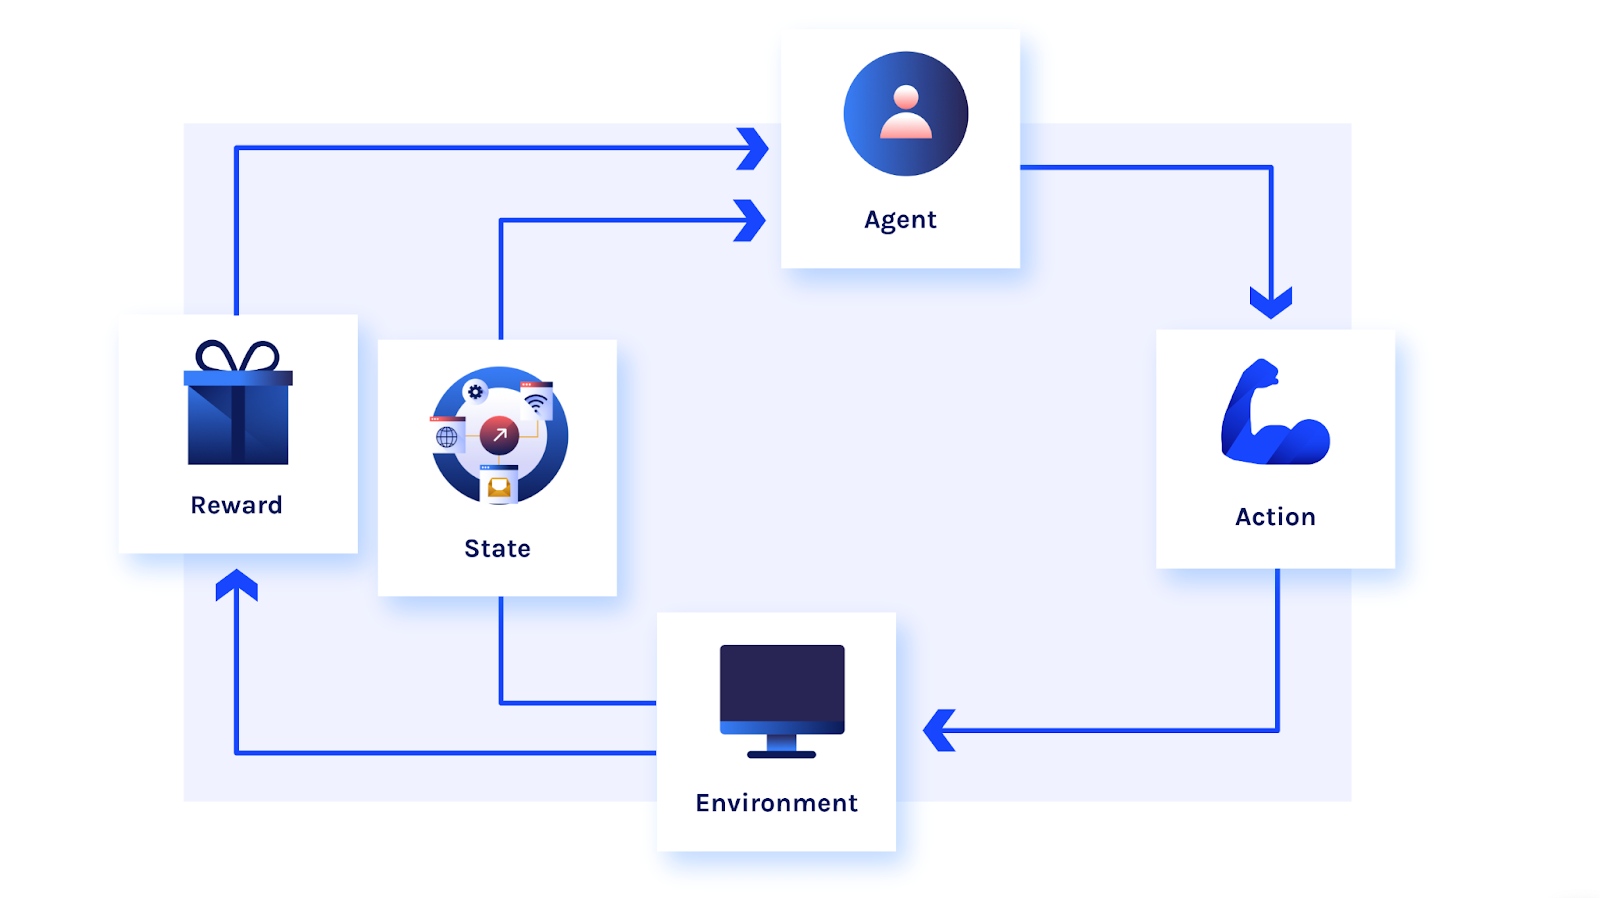
\includegraphics[height=6cm]{img/interaction-loop.png}
\\
\Large
\bold{Goal}: maximize the \textbf{cumulative reward} over time
\end{frame}

\begin{frame}{On problem expressiveness: reward hypothesis}
\begin{block}{Reward hypothesis}
\emph{Any goal can be formalized as the outcome of maximizing a cumulative reward}
\begin{itemize}
	\item Reinforcement learning is based on this hypothesis
	\item Ideally, we can formalize any problem as a reinforcement learning problem
\end{itemize}
\end{block}

\begin{alertblock}{Stronger statement: reward is enough}
\emph{intelligence, and its associated abilities, can be understood as subserving the maximisation of reward by an agent acting in its environment.}
\begin{itemize}
	\item Really controversial
\end{itemize}
\end{alertblock}
\end{frame}

\begin{frame}{Examples of Reinforcement Learning problems}
\begin{multicols}{2}
	\begin{itemize}
		\item Learning how to surf
		\item Managing a portfolio of cryptocurrencies
		\item Controlling the battery of an electric car 
		\item Playing chessboard
		\item Solving a cubic cube
	\end{itemize}
	\begin{itemize}
		\item[\faArrowRight] \textbf{Reward:} surfing time on the wave
		\item[\faArrowRight] \textbf{Reward:} money earned
		\item[\faArrowRight] \textbf{Reward:} battery level at the end of the day
		\item[\faArrowRight] \textbf{Reward:} win the game
		\item[\faArrowRight] \textbf{Reward:} solving time 
	\end{itemize}
\end{multicols}
\large
\textbf{NB!} if the goal is learn via environment interaction, then these are all reinforcement learning problems, regardless the algorithm involved
\end{frame}

\begin{frame}{Again, What is Reinforcement Learning}
\begin{itemize}
	\item There are several reasons why we should learn:
	\begin{enumerate}
		\item Find \textbf{solutions}
		\begin{itemize}
			\item A robot that reaches a target
			\item A program that plays chess (really well)
		\end{itemize}
		\item Adapt \textbf{online} (dealing with unknowns)
		\begin{itemize}
			\item A robot that learns how to walk in a new environment
			\item A program that learns how to play a new game
		\end{itemize}
	\end{enumerate}
	\item Reinforcement learning is used in both cases
	\item Episodic vs continuing tasks 

	\item Adapting online is more challenging, and it is not just generalization (e.g. supervised learning)
	\item Is it planning? \faArrowRight \, No, the \emph{model} is not known
\end{itemize}

\end{frame}

\begin{frame}{Motivating real world examples}
\centering
\href{https://www.youtube.com/watch?v=V1eYniJ0Rnk}{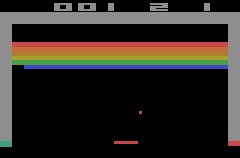
\includegraphics[width=0.32\textwidth]{img/atari.png}}
\href{https://www.youtube.com/watch?v=43cO39XBPIA}{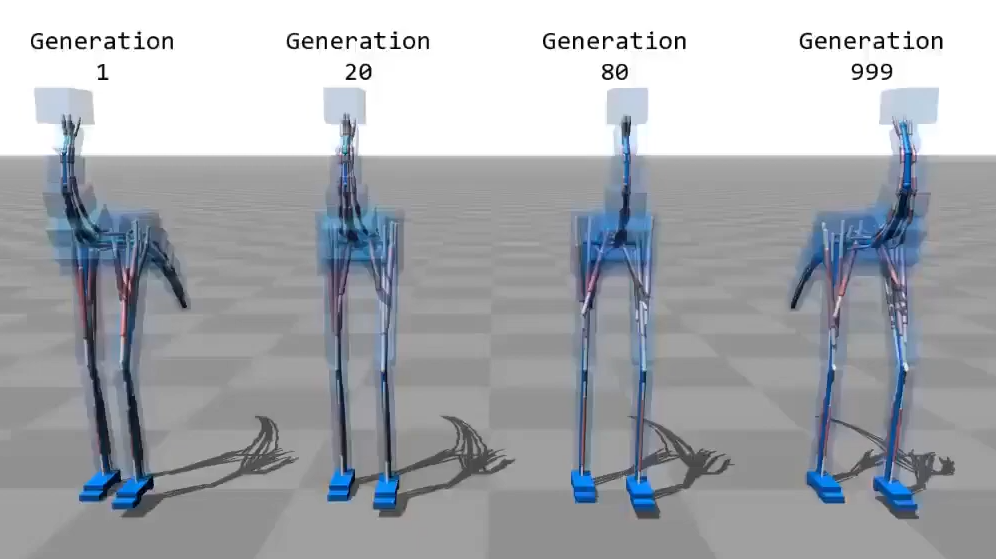
\includegraphics[width=0.32\textwidth]{img/robots.png}}
\href{https://www.youtube.com/watch?v=gn4nRCC9TwQ}{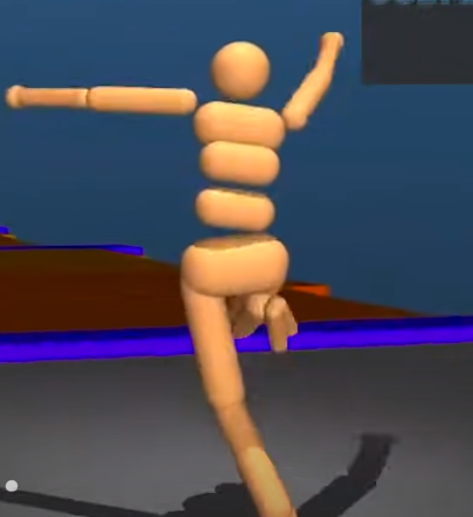
\includegraphics[width=0.32\textwidth]{img/ppo.png}}
\end{frame}
\section{Formalisation}
\begin{frame}{Reinforcement Learning: core concept}
Reinforcement learning formalism include:
\begin{itemize}
	\item \textbf{Environment}:
	\begin{itemize}
		\item Typically \emph{stochastic} and \emph{unknow} but \emph{stationary} (\textbf{Markov Decision Process})
		\item stochastic \faArrowRight \, the next state is \emph{not} fully determined by the current state and action (random component)
		\item Environment dynamics (i.e., the \emph{model}) expressed as: $p(s', r | s, a)$ \faArrowRight \, not known by the agent
	\end{itemize}
	\item \textbf{Reward signal} 
	\begin{itemize}
		\item Identifies what is \emph{good} in the environment (the goal)
	\end{itemize}
	\item \textbf{Agent}, which contain:
	\begin{itemize}	
		\item State
		\item Policy
		\item \emph{Value} function estimation?
	\end{itemize}
\end{itemize}
\end{frame}
\begin{frame}{Agent and environment}
\centering
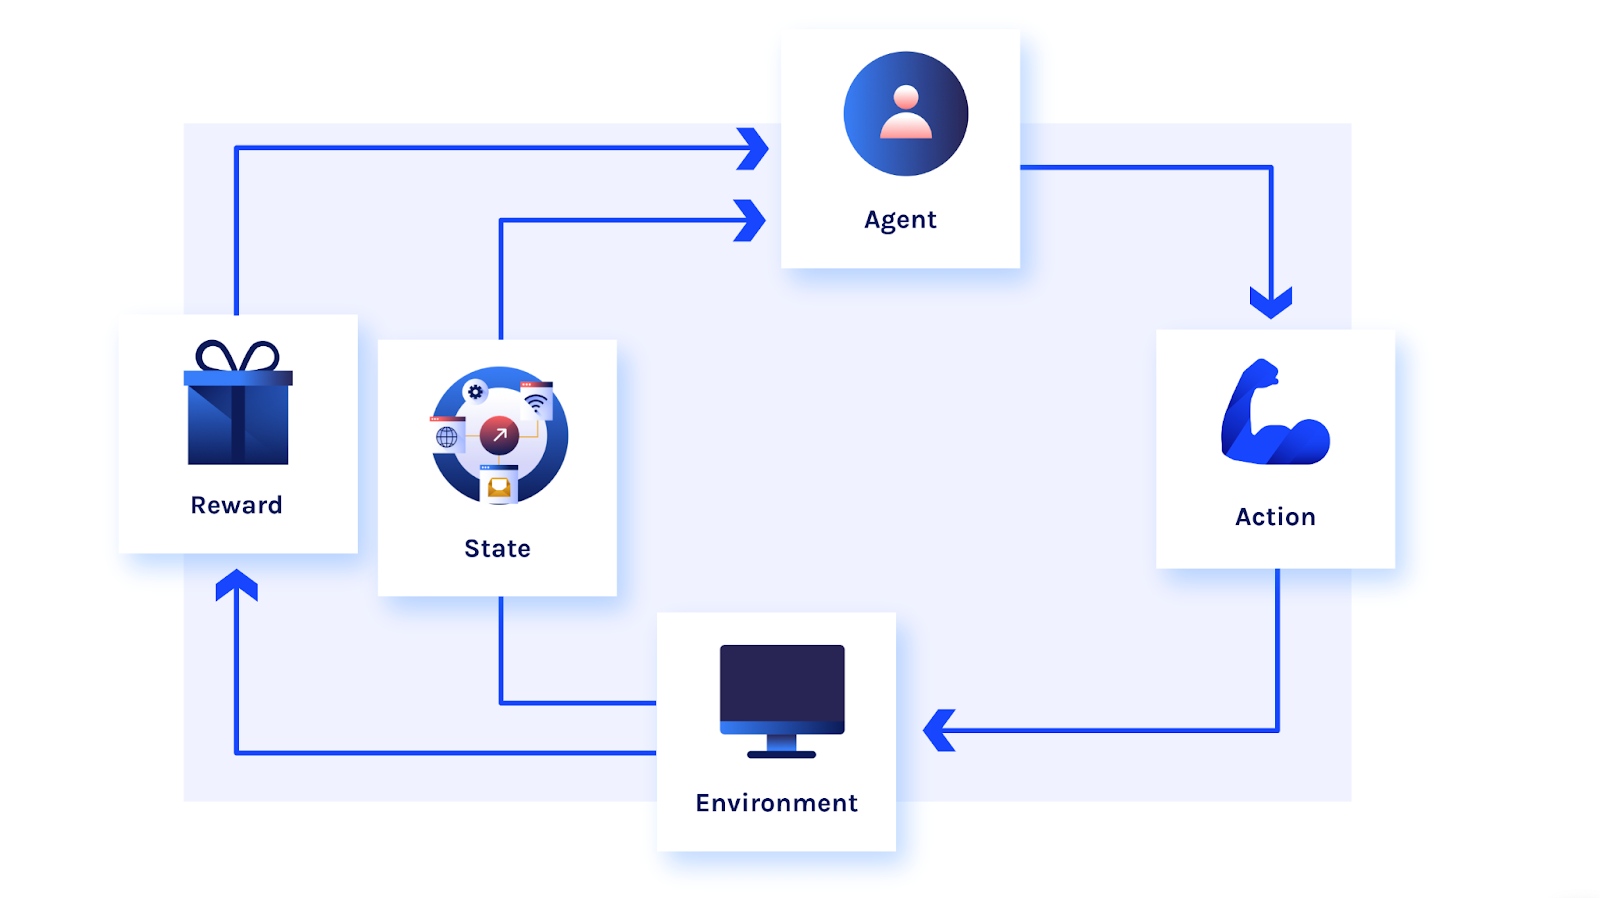
\includegraphics[height=4cm]{img/interaction-loop.png}
\begin{itemize}
	\item Each time step $t$:
	\begin{itemize}
		\item The agent receives an observation $s_t \in \mathcal{S}$ (and a reward $r_t \in \mathbb{R}$)
		\item Executes an action $a_t \in \mathcal{A}$
	\end{itemize}
	\item The environment 
	\begin{itemize}
		\item Receives the action $a_t$
		\item Emits the observation $s_{t+1}$ and the reward $r_{t+1}$
	\end{itemize}
\end{itemize}
\end{frame}
\begin{frame}{Agent state}
\begin{itemize}
	\item A full episode is a sequence of state-action-reward tuples (called \bold{trajectory})
	
	\item Example: $\mathcal{H}_T$ = $\{ (s_0, a_0, r_1), (s_1, a_1, r_2), \dots, (s_{T-1}, a_{T-1}, r_T) \}$
	\item Markovian property: the future is independent of the past given the present
	\begin{itemize}
		\item Formula: $p(s_{t+1} | s_t, a_t) = p(s_{t+1} | \mathcal{H}_t, a_t)$
		\item \textbf{NB!}: this means that the state $s_t$ is a \textbf{sufficient statistic} of the future
	\end{itemize}
	\item The environment state can be either:
	\begin{itemize}
		\item \textbf{Fully observable}: the agent knows the state
		\item \textbf{Partially observable}: the agent partially observes environment state 
	\end{itemize}
	\item Today we will assume that the state is \textbf{fully observable} and \textbf{Markovian}
	\item Real case scenario: \textbf{partially observable} and \textbf{non-Markovian}
	\begin{itemize}
		\item Also in that situation, reinforcement learning algorithms can be used (particularly the ones based on \emph{deep learning})
	\end{itemize}
\end{itemize}
\end{frame}
\begin{frame}{Example: Maze}
\centering
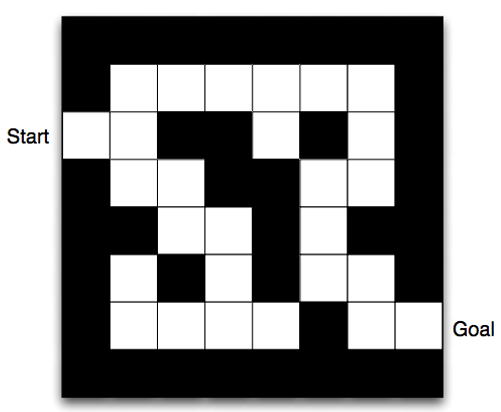
\includegraphics[width=0.48\textwidth]{img/maze.png}

\begin{itemize}
	\item \textbf{Action}: move in one of the four directions (up, down, left, right)
	\item \textbf{State}:\only<1>{\emph{???}} \only<2>{
		\emph{position in the maze}}
	\item \textbf{Reward}: \emph{???}
	\item \textbf{Policy}: \emph{???}
\end{itemize}
\end{frame}
\begin{frame}{Rewards}
\begin{itemize}
	\item A \bold{reward} $r_t$ is a scalar feedback signal
	\begin{itemize}
		\item In chess, $r_t = 1$ if the agent wins, $r_t = 0$ otherwise
		\item In a robot, $r_t = 1$ if the robot reaches the target, $r_t = 0$ otherwise
		\item For a portfolio, $r_t$ is the profit
	\end{itemize}
	\item Describes how well the agent is doing at step $t$ (define the goal)
	\item The agent's sole objective is to maximize the discounted cumulative reward (\bold{return})
	\begin{equation*}
	\begin{split}
		G_t & = r_{t+1} + \gamma r_{t+2} + \gamma^2 r_{t+3} + \dots \\
		 & = \sum_{k=0}^{\infty} \gamma^k r_{t+k+1}
		\end{split}
	\end{equation*}
\end{itemize}
\begin{alertblock}{Why discounted?}
\begin{itemize}
	\item Immediate rewards can be more important than future rewards
	\item $\gamma \in [0,1]$ is the discount factor
	\item $\gamma = 0$ \faArrowRight \, myopic agent
	\item $\gamma = 1$ \faArrowRight \, far-sighted agent
\end{itemize}
\end{alertblock}
\end{frame}
\begin{frame}{Example: Maze}
\centering
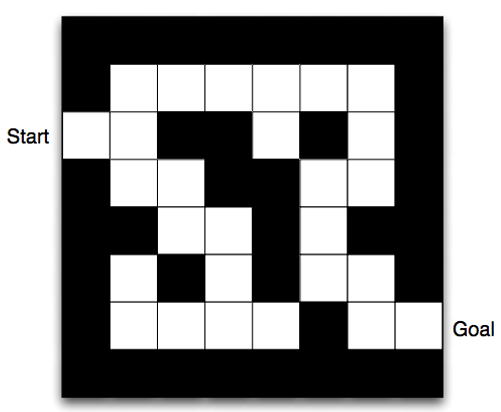
\includegraphics[width=0.5\textwidth]{img/maze.png}

\begin{itemize}
	\item \textbf{Action}: move in one of the four directions (up, down, left, right)
	\item \textbf{State}: \emph{position in the maze}
	\item \textbf{Reward}: 
	\begin{itemize}
		\item \emph{$r_t$ = -1 for each step, $r_t$ = 0 if the agent reaches the target}
		\item \emph{$r_t = 1$ if the agent reaches the target, $r_t = 0$ otherwise}
	\end{itemize}
	\item \textbf{Policy}: \emph{???}
\end{itemize}
\end{frame}
\begin{frame}{Agent Policy}
\begin{itemize}
	\item The agent's behavior is determined by a \bold{policy} $\pi$
	\item A policy is a mapping from state to action
	\item The policy can be either:
	\begin{itemize}
		\item \textbf{Deterministic}: $\pi: \mathcal{S} \rightarrow \mathcal{A}$
		\item \textbf{Stochastic}: $\pi: \mathcal{S} \times \mathcal{A} \rightarrow [0,1]$
	\end{itemize}
	\item The policy is typically represented as a \textbf{lookup table} or a \textbf{neural network}
	\item In both cases, the policy is based of an \textbf{estimation} of the \emph{value} function
\end{itemize}
\end{frame}
\begin{frame}{Example: Maze}
\centering
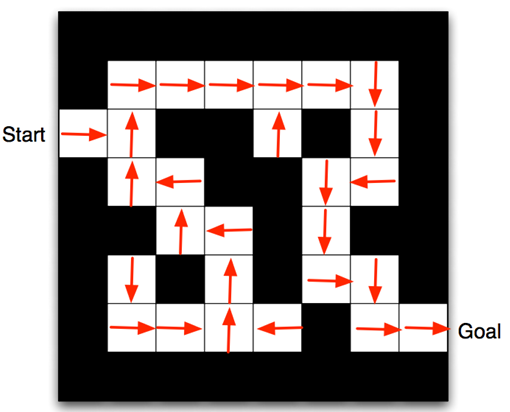
\includegraphics[width=0.48\textwidth]{img/shortest.png}
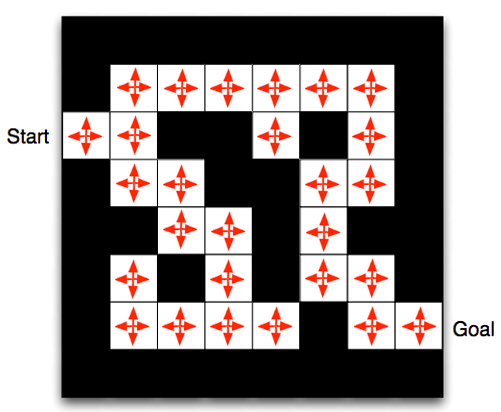
\includegraphics[width=0.48\textwidth]{img/maze-random.png}
\begin{itemize}
	\item \textbf{Action}: move in one of the four directions (up, down, left, right)
	\item \textbf{State}: \emph{position in the maze}
	\item \textbf{Reward}: 
	\begin{itemize}
		\item \emph{$r_t$ = -1 for each step, $r_t$ = 0 if the agent reaches the target}
		\item \emph{$r_t = 1$ if the agent reaches the target, $r_t = 0$ otherwise}
	\end{itemize}
	\item \textbf{Policy}: 
	\begin{itemize}
		\item \emph{shortest path to the target}
		\item \emph{random walk}
	\end{itemize}
\end{itemize}
\end{frame}
\begin{frame}{Value function}
\begin{itemize}
	\item The value function $v_{\pi}(s)$ gives the \textbf{long-term value} of state $s$ under policy $\pi$
	\item The value of a state is the total amount of reward an agent can expect to accumulate over the future, starting from that state
	\item Formally, it can be expressed as:
	\begin{equation*}
		\begin{split}
			v_{\pi}(s) = \mathbb{E}_{\pi} [G_t | S_t = s] = \mathbb{E}_{\pi} \left[ \sum_{k=0}^{\infty} \gamma^k r_{t+k+1} | S_t = s \right]	
		\end{split}
	\end{equation*}
	\item the state-action value function $q_{\pi}(s,a)$ gives the \textbf{long-term value} of state-action pair $(s,a)$ under policy $\pi$
	\begin{itemize}
		\item Formally, it can be expressed as:
		\begin{equation*}
			\begin{split}
				q_{\pi}(s,a) = \mathbb{E}_{\pi} [G_t | S_t = s, A_t = a] = \mathbb{E}_{\pi} \left[ \sum_{k=0}^{\infty} \gamma^k R_{t+k+1} | S_t = s, A_t = a \right]
			\end{split}
		\end{equation*}
	\end{itemize}
\end{itemize}
\end{frame}
\begin{frame}{Example: Maze (value)}
	\centering
	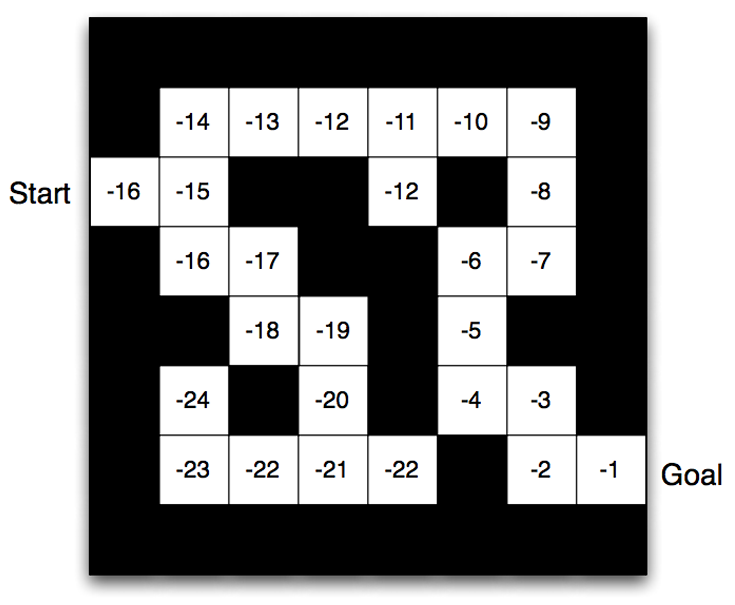
\includegraphics[width=0.8\textwidth]{img/value-maze.png}
\end{frame}
\begin{frame}{Bellman equation}
	\begin{itemize}
		\item The return $G_t$ can be computed recursively:
		\begin{equation*}
			\begin{split}
				G_t & = r_{t+1} + \gamma r_{t+2} + \gamma^2 r_{t+3} + \dots \\
				& = r_{t+1} + \gamma (r_{t+2} + \gamma r_{t+3} + \dots) \\
				& = r_{t+1} + \gamma G_{t+1} \\
			\end{split}
		\end{equation*}
		\item The value itself can be formulated recursively: 
		\begin{equation*}
			\begin{split}
			v_{\pi} & = \mathbb{E}_{\pi} [r_{t+1} + \gamma * G_{t+1} | S_t = s] \\
			& = \mathbb{E}_{\pi} [r_{t+1} + \gamma * v_{\pi}(s_{t+1}) | S_t = s] \\
			& = \sum_a \pi(a|s) \sum_{s'} \sum_r p(s', r | s, a) [r + \gamma G_{t+1}(s')]
			\end{split}
		\end{equation*}
		\item This is the \textbf{Bellman equation} and is the basis of many reinforcement learning algorithms (and ideas)
		\item A similar formulation can be be done for the optimal value function $v_*(s)$
		\begin{equation*}
			v^*(s) = max_a \mathbb{E} [r_{t+1} + \gamma * v_*(s_{t+1}) | S_t = s, A_t = a]
		\end{equation*}
		\item Can be also defined for the state-action value function $q^*(s,a)$
		\begin{equation*}
			q^*(s, a) = \mathbb{E} [r_{t+1} + \gamma * max_{a'} q^*(s_{t+1}, a') | S_t = s, A_t = a]
		\end{equation*}
	\end{itemize}
\end{frame}

\begin{frame}{Optimal policy}
\begin{itemize}
	\item The policy function can be defined on top of the value function (or the state-action value function)
	\item Greedy policy: $\pi_*(s) = argmax_a q_\pi(s,a)$ 
	\item Epsilon greedy policy: $\pi_*(s) = argmax_a q_\pi(s,a)$ with probability $1-\epsilon$, otherwise a random action is selected
	\item A policy $\pi$ is better than or equal to a policy $\pi'$ if its expected return is greater than or equal to that of $\pi'$ for all states
	\item The \emph{optimal} policy is the one that maximizes the expected return
	\item Formally, it can be expressed as:
	\begin{equation*}
		\pi_*(s) = argmax_a q_*(s,a)
	\end{equation*}
\end{itemize}
\end{frame}


\begin{frame}{Exploration vs Exploitation}
	\begin{itemize}
		\item \textbf{Exploration}: finds more information about the environment 
		\item \textbf{Exploitation}: exploits known information to maximize the reward 
		\item In order to find the optimal policy, the agent must explore the environment as well as exploit the knowledge it has already acquired
		\item This is the \textbf{exploration-exploitation dilemma}
		\item The agent must find a good trade-off between exploration and exploitation (e.g., $\epsilon$-greedy)
	\end{itemize}
\centering
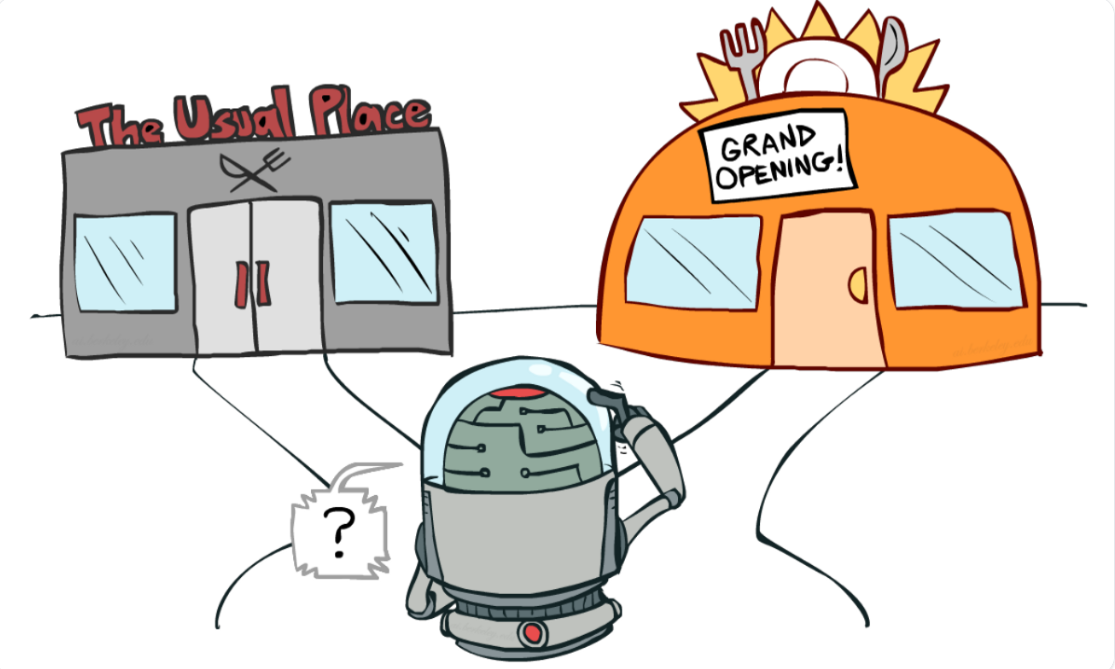
\includegraphics[width=0.5\textwidth]{img/exploration-exploitation.png}
\end{frame}
\begin{frame}{Recap -- modelling perspective}
\begin{exampleblock}<1-2>{Encode your application as a RL problem}
\begin{itemize}
	\item Identify the environment (i.e., the state space $\mathcal{S}$ of a given application)
	\item Identify the action space $\mathcal{A}$ of a given application (decisions that affect the state)
	\begin{itemize}
		\item \emph{Discrete} (e.g., chess)
		\item \emph{Continuous} (e.g., robot)
	\end{itemize}
	\item Identify the task type 
	\begin{itemize}
		\item \emph{Episodic}: the agent-environment interaction breaks down into episodes (e.g., chess)
		\begin{itemize}
			\item A sequence of actions that terminates in a terminal state
		\end{itemize}
		\item \emph{Continuing}: the agent-environment interaction continues without limit (e.g., robot)
	\end{itemize}
	\item Identify the reward function $r(s,a)$ (i.e., the goal of the application) 
\end{itemize}
\end{exampleblock}
\begin{alertblock}<2>{Find the optimal policy}
	\begin{itemize}
		\item Find the optimal policy $\pi_*$ that maximizes the expected return
		\item The optimal policy can be found by solving the Bellman equations \dots
		\item \dots but in practice it is not fleasible
		\begin{itemize}
			\item The model is not known
			\item Is computationally expensive
		\end{itemize}
	\end{itemize}
\end{alertblock}
\end{frame}
\section{Solving Reinforcement Learning problems}
\subsection{Tabular methods}
\begin{frame}{Optimal policy -- model based approach}
\begin{itemize}
	\item Simpliest approach: \textbf{policy iteration} (based on dynamic programming)
	\item Given a policy $\pi$:
	\begin{itemize}
		\item at each iteration, $k+1$
		\item For all states $s \in \mathcal{S}$:
		\item Evaluate the policy $\pi$ (i.e., compute $v_{\pi}(s) = \mathbb{E}[r_{t+1} + \gamma * {t+1} + ... | s_t = s]$)
		\item Improve the policy $\pi$ (i.e., compute $\pi'(s) = greedy(v_\pi)$)
	\end{itemize}
	\item In general, it nees to be repeated until convergence
	\item This process \emph{always} converges to the optimal policy
	\item Dynamic programming algorithms are based on this idea
\end{itemize}
\centering
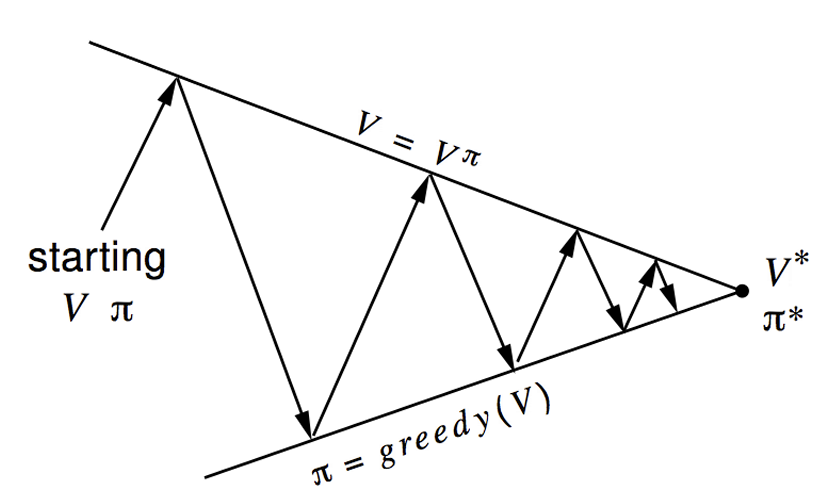
\includegraphics[width=0.5\textwidth]{img/policy-iteration.png}
\end{frame}
\begin{frame}{Model free approach -- families}
	\begin{itemize}
		\item \textbf{Value based}:
		\begin{itemize}
			\item Compute the value function and then derive the optimal policy (Q-learning, SARSA, DQN)
		\end{itemize}
		\item \textbf{Policy based}:
		\begin{itemize}
			\item Compute directly the optimal policy (REINFORCE)
		\end{itemize}
		\item \emph{Actor critic}:
		\begin{itemize}
			\item Have both a value function and a policy (A3C, PPO)
		\end{itemize}
	\end{itemize}
\end{frame}
\begin{frame}{Model-free approach -- Monte carlo}
	\begin{itemize}
		\item True essence of reinforcement learning: \textbf{trial and error}
		\item Simulated experience is used to solve the problem
		\item \textbf{Monte Carlo} methods are based on averaging sample returns
		\item How to guarentee that all states are visited?
	\end{itemize}
	\begin{alertblock}<1-2>{Monte carlo with exploring start (ES)}
		\begin{itemize}
			\item Start an arbitrary $\pi$ and $q$ and repeat forever the following steps:
			\begin{itemize}
				\item choose $s_0$ and $a_0$ such that all pairs have probability $> 0$
				\item generate an episode following $\pi$ (e.g., a simulation run)
				\item for each pair $s_t, a_t$ in the episode:
				\begin{itemize}
					\item $G \leftarrow$ return following the first occurence of $s_t, a_t$
					\item $q(s_t, a_t) \leftarrow average(G, q(s_t, a_t))$
					\item $\pi(s_t) \leftarrow argmax_a q(s_t, a)$
				\end{itemize}
			\end{itemize}
		\end{itemize}
	\end{alertblock}
	\begin{alertblock}<2>{Monte carlo with without ES}
		\begin{itemize}
			\item stick to an initial state $s_0$ 
			\item but be sure that all states will eventually be visited
			\item $\pi$ should never give less than $\epsilon > 0$ probability of being selected
			\item e.g., can super-impose current $\pi$ with a non-deterministic policy
		\end{itemize}
	\end{alertblock}
\end{frame}
\begin{frame}{Temporal difference (TD)}
	\begin{itemize}
		\item A combination of Monte Carlo ideas and dynamic programming ideas
		\item Like Monte Carlo methods, TD methods can learn directly from raw experience without a model of the environment's dynamics
		\item Like dynamic programming methods, TD methods update estimates based in part on other learned estimates, without waiting for a final outcome (they \emph{bootstrap})
		\begin{itemize}
			\item bootstrap:  value of a state is updated based on the estimated value of the next state
		\end{itemize}
	\end{itemize}
	\begin{exampleblock}{Example methods}
		\begin{itemize}
			\item Q-Learning: updates q using next state and $\epsilon-greedy$ policy for current q (\emph{off-policy})
			\item SARSA: updates q using next state and $\epsilon-greedy$ policy for next q (\emph{on-policy})
		\end{itemize}
	\end{exampleblock}
	\begin{alertblock}{Q-learning}
		\begin{itemize}
			\item Generally considered a flexble, simple and effective method: typically the starting point
		\end{itemize}
	\end{alertblock}
\end{frame}
\begin{frame}{Q-learning}
	\begin{exampleblock}<1-2>{Algorithm core: Q-update}
		\begin{itemize}
			\item $ q(s_t, a_t) = (1 - \alpha) * q(s_t, a_t) + \alpha [r_{t+1} + \gamma * max_a \, q(s_{t+1}, a)] $
			\item $\alpha$ is the \emph{learning rate} ($\alpha \in [0,1]$)
			\item it is proven that this converges to the optimal q function (if $\alpha$ is sufficiently small and all state-action pairs are visited infinitely often)
		\end{itemize}
	\end{exampleblock}
	\begin{alertblock}<2>{Full algorithm (episodic task)}
		\begin{itemize}
			\item initialize Q arbitrarily, and put 0 on terminal states
			\item for each episode:
			\item initialize $s_0$ (e.g., randomly) and $t = 0$
			\begin{itemize}
				\item for each step t:
				\begin{enumerate}
					\item choose $a_t$ from $s_t$ using a policy from q (e.g., $\epsilon-greedy$)
					\item take the action $a_t$ and observe $r_t$, $s_{t+1}$ (interaction with the environment)
					\item perform the update $q(s_t, a_t) = (1 - \alpha) * q(s_t, a_t) + \alpha [r_{t+1} + \gamma * max_a \, q(s_{t+1}, a)] $
					\item increase $t$
					\item end if $s_{t+1}$ is terminal (or $t > T$)
				\end{enumerate}
			\end{itemize}
		\end{itemize}
	\end{alertblock}
\end{frame}
\begin{frame}{Q-learning -- pratical tips}
	\begin{exampleblock}<1-2>{Exploration-exploitation trade-off}
		\begin{itemize}
			\item $\epsilon-greedy$ policy is a simple way to balance exploration and exploitation
			\item Typically, is better to start with a high $\epsilon$ and then decrease it over time
			\item This is called \emph{$\epsilon$-decay} and can be done in different ways
			\item Example (linear decay): $\epsilon = max(\epsilon_{min}, \epsilon_{max} - \frac{t}{\epsilon_{decay}})$
			\item Example (exponential decay): $\epsilon = \epsilon_{min} + (\epsilon_{max} - \epsilon_{min}) * e^{-\lambda * t}$
		\end{itemize}		
	\end{exampleblock}
	\begin{exampleblock}<2>{Learning rate}
		\begin{itemize}
			\item Learning rate $\alpha$ is typically set to a small value (e.g., 0.1)
			\item However, it can be useful to decrease it over time 
			\item \textbf{Motivation}: the agent can learn faster in the beginning and then slow down the learning rate
			\item Example (linear decay): $\alpha = max(\alpha_{min}, \alpha_{max} - \frac{t}{\alpha_{decay}})$
		
		\end{itemize}
	\end{exampleblock}
\end{frame}
\begin{frame}{Q-learning -- Offline and online applications}
\begin{exampleblock}<1-2>{Offline}
	\begin{itemize}
		\item create a simulation of the selected environment (e.g., a trading simulator)
		\item simulate the agent-environment interaction learning the Q-function
		\item in production use the learned Q-function to take decisions
		\item \textbf{cons}: 
		\begin{itemize}
			\item no adaptation to the real environment
			\item the simulation must be a good approximation of the real environment
		\end{itemize}
	\end{itemize}
\end{exampleblock}
\begin{alertblock}<2>{Online}
	\begin{itemize}
		\item learn the Q-function while interacting with the real environment
		\item implement your agent and let it learn while taking decisions
		\item pratical solution: initially learn fast and then slow down the learning rate
		\item \textbf{cons}:
		\begin{itemize}
			\item the agent can take bad decisions while learning (e.g., the robot can fall)
			\item the agent can take a lot of time to learn
		\end{itemize}
	\end{itemize}
\end{alertblock}
\end{frame}

\begin{frame}{Q-learning -- programming perspective}
	\begin{itemize}
		\item What is the best way to implement Q-learning? (or in general RL algorithms)
		\item \bold{Separation of concerns}:
		\begin{itemize}
			\item \textbf{Environment}: the environment is a black box that can be interacted with (e.g., a trading simulator)
			\begin{itemize}
				\item Role: provide a clear interface to the agent in order to interact with the environment
				\item Reference example: gymnasium: \url{https://gymnasium.farama.org/}
			\end{itemize}
			\item \textbf{Policy}: the policy is a function that maps states to actions
			\begin{itemize}
				\item It could be a lookup table or a neural network
				\item In the case of a neural network, there is a need of autodifferentiation library
				\item State-of-the-art libraries: \bold{PyTorch} (\url{https://pytorch.org/}), \bold{Tensorflow} (\url{https://www.tensorflow.org/}), and \bold{TorchRL} (\url{https://github.com/pytorch/rl})
			\end{itemize}
			\item \textbf{Learning algorithm}: the learning algorithm is responsible for learning the policy
			\begin{itemize}
				\item It could be a simple algorithm (e.g., Q-learning) or a complex one (e.g., DQN)
				\item Some libraries provide a set of algorithms: Stable Baselines (\url{https://stable-baselines3.readthedocs.io/en/master/})
			\end{itemize}
		\end{itemize}
	\end{itemize}
	\centering 
	\Large Hands-on at \url{todo}
\end{frame}
\subsection{Approximate methods -- Deep Reinforcement Learning}
%\subsection{Reinforcement Learning Pitfalls}
\begin{frame}{Reinforcement Learning Pitfalls: Large state space}
\begin{block}{Problem}
	\begin{itemize}
		\item \textbf{State space} \faArrowRight \, set of all possible states
		\item \textbf{State space explosion} \faArrowRight \, the number of states is too large to be stored in memory
	\end{itemize}
\end{block}
\begin{columns}
	\begin{column}{0.5\textwidth}
		
			\begin{block}{Example (Go) \, \href{}{\faLink}}
				\begin{itemize}
					\item $10^{170}$ possible states \bold{(!!!!)}
					\item $10^{80}$ atoms in the universe
					\item $10^{16}$ seconds since the Big Bang
				\end{itemize}
			\end{block}
			\begin{block}{Example (Chess) \, \href{}{\faLink}}
				\begin{itemize}
					\item $10^{46}$ possible states
					\item total space required $\sim$ $10^{35}$ terabytes
				\end{itemize}
			\end{block}
	\end{column}
	\begin{column}{0.5\textwidth}
	\centering
	\fbox{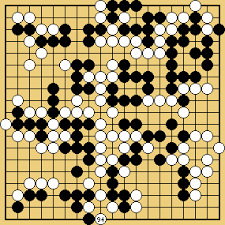
\includegraphics[width=0.67\linewidth]{img/go.png}}
	\end{column}
\end{columns}

\begin{alertblock}{Question}
	\centering
	\textbf{How to deal with large state space?}
\end{alertblock}
\end{frame}

\begin{frame}{Reinforcement Learning Pitfalls: Continous Action Space}
	\begin{block}{Problem}
		\begin{itemize}
			\item \textbf{Action space} \faArrowRight \, set of all possible actions
			\item \textbf{Continous action space} \faArrowRight \, the actions are real numbers (e.g. $[0,1]$) \faArrowRight infinite number of actions
		\end{itemize}
	\end{block}
	\begin{columns}
		\begin{column}{0.5\textwidth}
			\begin{block}{Example (Robotics) \, \href{}{\faLink}}
				\begin{itemize}
					\item \textbf{Action space} \faArrowRight \, the set of all possible joint angles
					\item \textbf{Continous action space} \faArrowRight \, the set of all possible real joint angles
				\end{itemize}
			\end{block}
		\end{column}
		\begin{column}{0.5\textwidth}
			\centering
			\fbox{
\includegraphics[width=0.4\linewidth]{img/robotics}}
		\end{column}
	\end{columns}
	
	\begin{alertblock}{Question}
		\centering
		\textbf{How to deal with continous action space?}
	\end{alertblock}
\end{frame}
\begin{frame}{Reinforcement Learning Pitfalls: Generalization}
\begin{block}{Problem}
	\begin{itemize}
		\item \textbf{Generalization} \faArrowRight \, the ability to perform well on previously unseen environments
		\item Can be also seen as \textbf{transfer learning} \faArrowRight \, the ability to transfer knowledge from one environment to another
		\item \textbf{Generalization gap} \faArrowRight \, the difference between the performance on the training environments and the performance on the test environments
	\end{itemize}
\end{block}
\begin{block}{Example (Go) \, \href{}{\faLink}}
	\begin{itemize}
		\item \textbf{Generalization} \faArrowRight \, the ability to play well with different opponents
		\item \textbf{Generalization gap} \faArrowRight \, the difference between the performance on the training set and the performance on the test set
	\end{itemize}
\end{block}
\begin{alertblock}{Question}
	\centering
	\textbf{How to deal with generalization?}
\end{alertblock}
\end{frame}
%\subsection{Deep Reinforcement Learning Overview}
\begin{frame}{Deep Reinforcement Learning}
	\centering
	\fbox{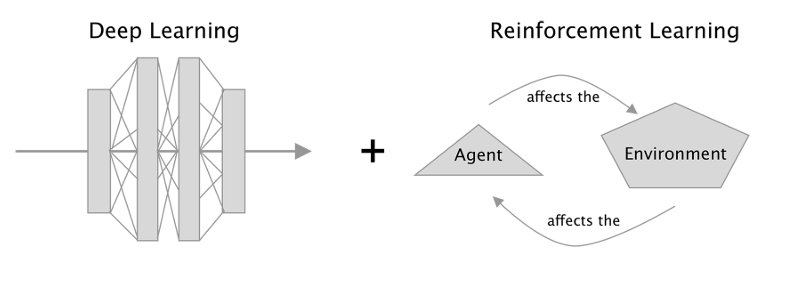
\includegraphics[width=0.7\textwidth]{img/deep-rl.png}}
	\begin{block}{Overview}
		\begin{itemize}
			\item \textbf{Deep Reinforcement Learning (DRL)} \faArrowRight \, the use of deep neural networks to approximate the value function / policy
			%\item Stochastic gradient descent \faArrowRight \, the use of gradient descent to train the neural networks
		\end{itemize}
	\end{block}
	
	\begin{alertblock}{Key features}
		\begin{itemize}
			\item \textbf{value function approximation} (instead of table) \faArrowRight \, \textbf{handle large state space}
			\item \textbf{policy gradient} (instead of Q-Learning) \faArrowRight \, \textbf{handle continous action space}
			\item \textbf{deep neural networks} \faArrowRight \, \textbf{handle generalization} (Representation learning)
		\end{itemize}
	\end{alertblock}
\end{frame}
\begin{frame}{Deep Q-Learning}
	\centering
	\textbf{Q-Learning but q-function is approximated by a neural network}
	$$ Q(s, a, \theta) \sim Q(s, a) $$
	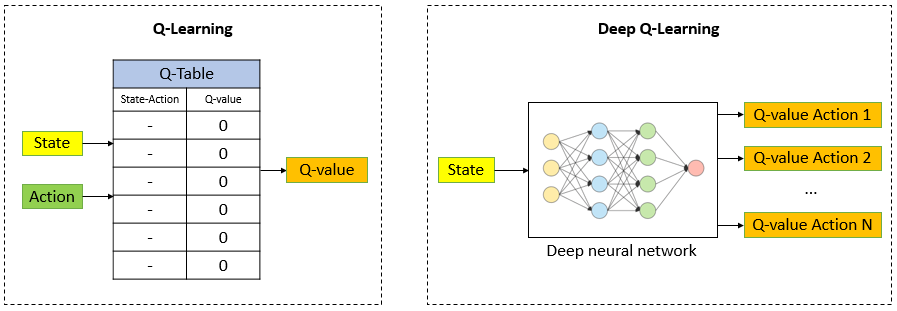
\includegraphics[width=\textwidth]{img/dql-vs-ql-1.png}
\end{frame}

\begin{frame}{Deep Q-Learning}
	\begin{alertblock}{Loss function}
		\begin{itemize}
			\item Bellman equation: $Q(s, a) = (r + \gamma \max_{a'} Q(s', a'))$
			\item Treating $r + \gamma \max_{a'} Q(s', a')$ as a target value
			\item Regression problem: $L(\theta) = (r + \gamma \max_{a'} Q(s', a', \theta) - Q(s, a, \theta))^2$
		\end{itemize}
	\end{alertblock}
	\begin{block}{Issues}
		\begin{itemize}
			\item \textbf{Correlation} \faArrowRight \, the samples are not independent
			\item \textbf{Non-stationary} \faArrowRight \, the target value changes over time
		\end{itemize}
	\end{block}
	\begin{alertblock}{Solutions}
		\begin{itemize}
			\item \textbf{Replay Buffer} \faArrowRight \, store the transitions $(s, a, r, s')$ and sample them randomly
			\item \textbf{Target Network} \faArrowRight \, used to compute the target value
		\end{itemize}
	\end{alertblock}
\end{frame}
\begin{frame}{Deep Q Learning: Replay Buffer}
	\centering
	\fbox{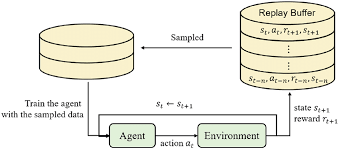
\includegraphics[width=0.5\textwidth]{img/replay-buffer.png}}
	\begin{block}{How}
		\begin{itemize}
			\item Store the transitions $(s, a, r, s')$ in $\mathcal{D}$ of prior experience
			\item During Backpropagation, sample a batch of transitions $(s, a, r, s')$ 
		\end{itemize}
	\end{block}
	\begin{block}{Loss computation}
		\begin{itemize}
			\item Sample a random batch of transitions $(s, a, r, s')$ from $\mathcal{D}$
			\item Compute the target value $y = r + \gamma \max_{a'} Q(s', a', \theta)$
			\item Use the target value to compute the loss $L(\theta) = \mathbb{E}[(y - Q(s, a, \theta))^2]$
		\end{itemize}
	\end{block}
\end{frame}
\begin{frame}{Deep Q Learning: Fixed Target Network}
	\centering
	%\fbox{\includegraphics[width=0.5\textwidth]{img/target-network.png}}
	\begin{block}{How}
		\begin{itemize}
			\item Use a separate network to compute the target value
			\item The target network is updated every $C$ steps
		\end{itemize}
	\end{block}
	\begin{block}{Loss computation}
		\begin{itemize}
			\item Let $\theta^-$ be the parameters of the target network
			\item Sample a random batch of transitions $(s, a, r, s')$ from $\mathcal{D}$
			\item Compute the target value $y = r + \gamma \max_{a'} Q(s', a', \theta^-)$
			\item Use the target value to compute the loss $L(\theta) = \mathbb{E}[(y - Q(s, a, \theta))^2]$
			\item After $C$ steps, update the target network parameters $\theta^- \leftarrow \theta$
		\end{itemize}
	\end{block}
	\begin{alertblock}{Benefits}
		\begin{itemize}
			\item \textbf{Stable} \faArrowRight \, the target value is fixed for $C$ steps, avoiding the non-stationary issue (dipendece on target and prediction cause)
		\end{itemize}
	\end{alertblock}
\end{frame}
\begin{frame}{Deep Q Learning: Epsilon decay}
	\begin{block}{How}
		\begin{itemize}
			\item $\epsilon$ is the probability of selecting a random action
			\item $\epsilon$ is decayed over time (or steps or episodes)
			\item \textbf{(!!!)} Off-policy nature of DQL \faArrowRight \, the agent can learn from random actions
		\end{itemize}
	\end{block}
	\begin{block}{Why}
		\begin{itemize}
			\item \textbf{Exploration vs Exploitation} \faArrowRight \, the agent needs to explore the environment to learn the optimal policy
			\item \textbf{Exploitation} \faArrowRight \, the agent needs to exploit the learned policy to maximize the reward
		\end{itemize}
	\end{block}
	
\end{frame}
\begin{frame}{Deep Q Learning: Algorithm}
	\begin{block}{Algorithm}
		\begin{itemize}
			\item Initialize the replay buffer $\mathcal{D}$
			\item Initialize the target network parameters $\theta^-$
			\item Initialize the Q-network parameters $\theta$
			\item \textbf{for} episode = 1, M \textbf{do}
			\begin{itemize}
				\item Initialize the initial state $s_1$
				\item \textbf{for} t = 1, T \textbf{do}
				\begin{itemize}
					\item With probability $\epsilon$ select a random action $a_t$
					\item otherwise select $a_t = argmax_a Q(s_t, a, \theta)$
					\item Execute action $a_t$ in the environment and observe reward $r_t$ and next state $s_{t+1}$
					\item Store transition $(s_t, a_t, r_t, s_{t+1})$ in $\mathcal{D}$
					\item Sample a random minibatch of transitions $(s, a, r, s')$ from $\mathcal{D}$
					\item Set $y_i = r + \gamma \max_{a'} Q(s', a', \theta^-)$
					\item Perform a gradient descent step on $(y_i - Q(s, a, \theta))^2$ with respect to the network parameters $\theta$
					\item Every $C$ steps reset $\theta^- \leftarrow \theta$
				\end{itemize}
			\end{itemize}
		\end{itemize}
	\end{block}
\end{frame}
\begin{frame}{Deep Q Learning: Extensions and Limits}
	\begin{block}{Limits}
		\begin{itemize}
			\item Works only for discrete action spaces
			\item Sample inefficiencient
			\item Overestimation of the action value due to the max operator
		\end{itemize}
	\end{block}
	\begin{block}{Extensions}
		\begin{itemize}
			\item \textbf{Double DQN} \faArrowRight \, use two separate networks to select and evaluate the action
			\begin{itemize}
				\item Pro: avoid overestimation of the action value
			\end{itemize}
			%\item \textbf{Dueling DQN} \faArrowRight \, use two separate networks to estimate the state value and the advantage function
			%\begin{itemize}
		%		\item Pro: better estimation of the action value
		%	\end{itemize}
			\item \textbf{Prioritized Experience Replay} \faArrowRight \, sample the transitions from the replay buffer according to their TD-error
			\begin{itemize}
				\item Pro: better exploration of the state space
			\end{itemize}
			\item \textbf{Raindow DQN} \faArrowRight \, combination of the previous extensions
		\end{itemize}
	\end{block}
\end{frame}

\begin{frame}{Policy gradient methods -- REINFORCE}
	\begin{itemize}
		\item \textbf{Policy gradient} \faArrowRight \, the policy is directly optimized
		\item \bold{REINFORCE} is an policy gradient algorithm for maximizing the expected return $G = \sum_{t=0}^T \gamma^t r_t$
		\item \emph{intuition}: trial and error
		\begin{itemize}
			\item Sample a trajectory $\tau$ from the policy $\pi(\theta$). If the trajectory is good, increase the probability of the actions. Otherwise, decrease the probability of the actions
			\item It can be seen as stochasti gradient ascent on $G(\H_T)$
		\end{itemize}
		\item we want train the policy in a way thata:
		\begin{equation*}
			\theta_{n+1} = \theta_{n} + \alpha \nabla J(\theta_n)
		\end{equation*}
		\item where $J(\theta) = \mathbb{E}_{\pi(\theta)}[G]$
	\end{itemize}
\end{frame}	
\begin{frame}{Policy gradient methods -- REINFORCE (cont.)}
\begin{itemize}
	\item Maximize $ \mathbb{E}_{\pi(\theta)}[G]$ with gradient ascent:
	\begin{equation*}
		\nabla_\theta \mathbb{E}_{\pi(\theta)}[G] = \nable_\theta \int G
	\end{equation*}
\end{itemize}
\end{frame}
%===============================================================================
\section*{}
%===============================================================================

%/////////
\frame{\titlepage}
%/////////

%===============================================================================
\section*{\refname}
%===============================================================================

%%%%
\setbeamertemplate{page number in head/foot}{}
%/////////


%%%%%%%%%%%%%%%%%%%%%%%%%%%%%%%%%%%%%%%%%%%%%%%%%%%%%%%%%%%%%%%%%%%%%%%%%%%%%%%%
\end{document}
%%%%%%%%%%%%%%%%%%%%%%%%%%%%%%%%%%%%%%%%%%%%%%%%%%%%%%%%%%%%%%%%%%%%%%%%%%%%%%%%
